\subsection{Task 1.1.4: Regularized Polynomial Regression}

%nöhmes stuff:

\paragraph{Regularized Regression Grundlagen}

Folgende Fehlerfunktion soll minimal werden:

$$ E(\vect{w}) = \frac{1}{N} \sum_{i=1}^N(y_i - \sum_{k=1}^d \Phi_k(x_i) w_k)^2 + \alpha^2 \sum_{k=1}^d w_k^2 $$

Zuerst müssen die indizierten Variablen in Vektoren umgeschrieben werden:

$$ \vect{x} = \begin{bmatrix} x_1 \\ x_2 \\ \vdots \\ x_N \end{bmatrix}, \; \vect{y} = \begin{bmatrix} y_1 \\ y_2 \\ \vdots \\ y_N \end{bmatrix}, \; \vect{w} = \begin{bmatrix} w_1 \\ w_2 \\ \vdots \\ w_d \end{bmatrix}, \; \vect{\Phi}(\vect{x}) = \begin{bmatrix} \Phi_1(\vect{x}) \\ \Phi_2(\vect{x}) \\ \vdots \\ \Phi_d(\vect{x}) \end{bmatrix} $$

wobei $ \vect{x} \in M(N \times 1), \; \vect{y} \in M(N \times 1), \; \vect{w} \in M(d \times 1), \; \vect{\Phi}(\vect{x}) \in M(d \times 1) $.

Nun können die Summen in Matrixform umgeschrieben werden (von innen nach aussen):

$$ \sum_{k=1}^d \Phi_k w_k = \vect{\Phi}^T \cdot \vect{w}, \; \text{da} \begin{bmatrix} \Phi_1 && \Phi_2 && \hdots && \Phi_d \end{bmatrix} \cdot \begin{bmatrix} w_1 \\ w_2 \\ \vdots \\ w_d \end{bmatrix} = \Phi_1 w_1 + \Phi_2 w_2 + \hdots + \Phi_d w_d \; \text{(Skalar)} $$

$$ \alpha^2 \sum_{k=1}^d w_k^2 = \alpha^2 \cdot \vect{w}^T \cdot \vect{w}, \; \text{aus dem selben Grund wie oben (ebenfalls Skalar)} $$

Mit der gleichen Regel kann man auch die äußere Summe zusammenfassen:

$$ \sum_{i=1}^N (y_i - \sum_{k=1}^{d} \Phi_k(x_i) w_k)^2 = (\vect{y} - \vect{\Phi}(\vect{x})^T \vect{w})^T (\vect{y} - \vect{\Phi}(\vect{x})^T \vect{w}), \; \text{dim} = (N \times d) $$

Also ergibt sich die gesamte Fehlerfunktion als:

$$ E(\vect{w}) = \frac{1}{N} (\vect{y} - \vect{\Phi}(\vect{x})^T \vect{w})^T (\vect{y} - \vect{\Phi}(\vect{x})^T \vect{w}) + \alpha^2 \vect{w}^T \vect{w} \; \text{(Skalar)} $$

Die Matrix $ \vect{\Phi}(\vect{x})^T $ wird im folgenden als Designmatrix $ \vect{X} $ abgekürzt und hat folgende Form:

$$ \vect{X} = \vect{\Phi}(\vect{x})^T = \begin{bmatrix} \Phi_1(x_1) && \Phi_2(x_1) && \hdots && \Phi_d(x_1) \\  \Phi_1(x_2) && \Phi_2(x_2) && \hdots && \Phi_d(x_2) \\ \vdots && \ddots \\ \Phi_1(x_N) && \Phi_2(x_N) && \hdots && \Phi_d(x_N) \end{bmatrix} $$

Ihre Dimension ist also $ \vect{X} \in M(N \times d) $.

Um nun den Fehler zu minimieren, muss die Fehlerfunktion abgeleitet werden:

$$ \frac{\partial E(\vect{w})}{\partial \vect{w}} = \frac{\partial}{\partial \vect{w}} \frac{1}{N} (\vect{y} - \vect{X} \vect{w})^T (\vect{y} - \vect{X} \vect{w}) + \alpha^2 \vect{w}^T \vect{w} $$

Mit $ \frac{\partial \vect{w}^T \vect{w}}{\partial \vect{w}} = 2 \vect{w}^T $ (Matrix-Cookbook, (10)) ergibt sich (innere Ableitung nicht vergessen!):

$$ \frac{\partial E(\vect{w})}{\partial \vect{w}} = - \frac{2}{N} (\vect{y} - \vect{X} \vect{w})^T \vect{X} + 2 \alpha^2 \vect{w}^T $$

Um das Minimum zu finden, wird diese Ableitung jetzt 0 gesetzt und auf $\vect{w}$ umgeformt:

$$ - \frac{2}{N} (\vect{y} - \vect{X} \vect{w})^T \vect{X} + 2 \alpha^2 \vect{w}^T = 0 $$
$$ \frac{2}{N} (\vect{y} - \vect{X} \vect{w})^T \vect{X} = 2 \alpha^2 \vect{w}^T $$
$$ (\vect{y} - \vect{X} \vect{w})^T \vect{X} = N \alpha^2 \vect{w}^T $$
$$ (\vect{y}^T - \vect{w}^T \vect{X}^T) \vect{X} = N \alpha^2 \vect{w}^T $$
$$ \vect{y}^T \vect{X} - \vect{w}^T \vect{X}^T \vect{X} = N \alpha^2 \vect{w}^T $$
$$ \vect{w}^T \vect{X}^T \vect{X} + N \alpha^2 \vect{w}^T = \vect{y}^T \vect{X} $$
$$ \vect{w}^T \vect{X}^T \vect{X} + \vect{w}^T N \alpha^2 = \vect{y}^T \vect{X} $$
$$ \vect{w}^T (\vect{X}^T \vect{X} + N \alpha^2 \vect{I}) = \vect{y}^T \vect{X} $$
$$ \vect{w}^T = \vect{y}^T \vect{X} (\vect{X}^T \vect{X} + N \alpha^2 \vect{I})^{-1} $$
$$ \vect{w} = (\vect{X}^T \vect{X} + N \alpha^2 \vect{I})^{-1} \vect{X}^T \vect{y} $$
%endlich!!! :)


%tom stuff:



\paragraph{Polynomial Basis Functions}


Wie in der Abbildung \ref{fig:poly_mse} zu sehen ist, ergibt sich ein minima des MSE der Testdaten
bei $\alpha = 0.00015167$. Wie in der Abbildug \ref{fig:poly_learned} zu sehen ist, bewirkt ein höherer Wert von
$\alpha$ ein Abflachen der Lernkurve. Bei kleineren Werten von $\alpha$ ist die Kurve weniger abgeflacht und
folgt mehr den Trainigsdaten. Ein kleinerer Wert von $\alpha$ hat jedoch den entscheidenden Nachteil, dass ausserhalb
des Bereichs der Trainingsdaten(auf der x-Achse), die Lernkurve sehr stark nach oben bzw. unten wegknickt.
$\alpha$ vergrößert bei größeren Gewichten die Fehlerfunktion $E(x)$ und wirkt somit dem entgegen.

Der mean squared error korrelliert sehr gut dem Mittelwert der absoluten Gewichte. Für Größere Werte von $\alpha$
ergibt sich verbessert sich der MSE bei den Trainings- und Testdaten. Wird jedoch $\alpha$ zu groß gewählt, so steigt
der MSE wieder.


  \begin{center}
	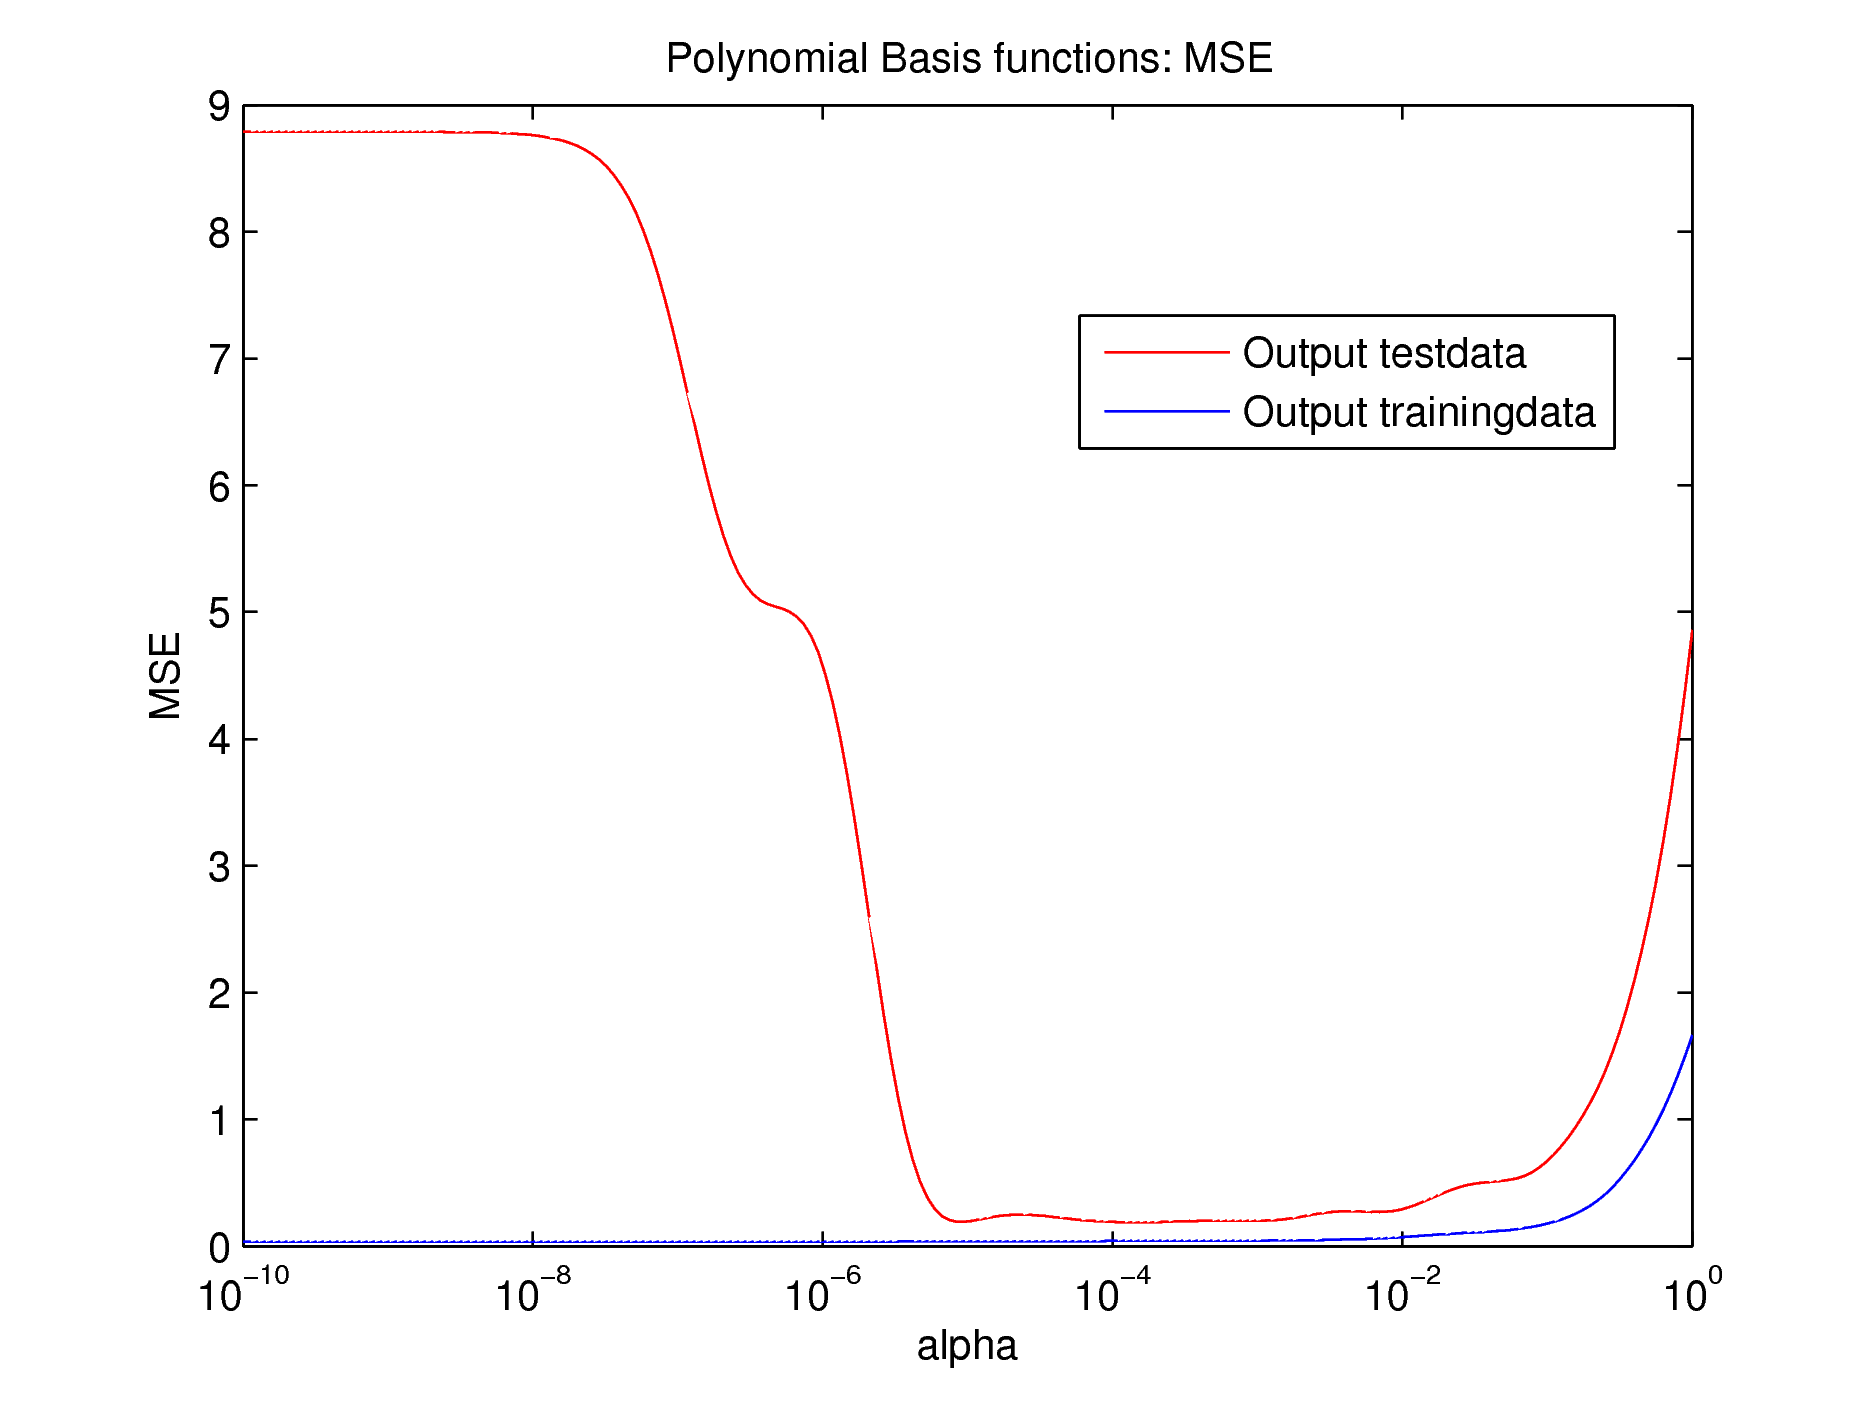
\includegraphics[width=15cm]{figures/114/poly_mse.png}
	\captionof{figure}{Polynomial Basis Functions: Mean squared error, Minimum bei $\alpha = 0.00015167$}
	\label{fig:poly_mse}
  \end{center}

  \begin{center}
	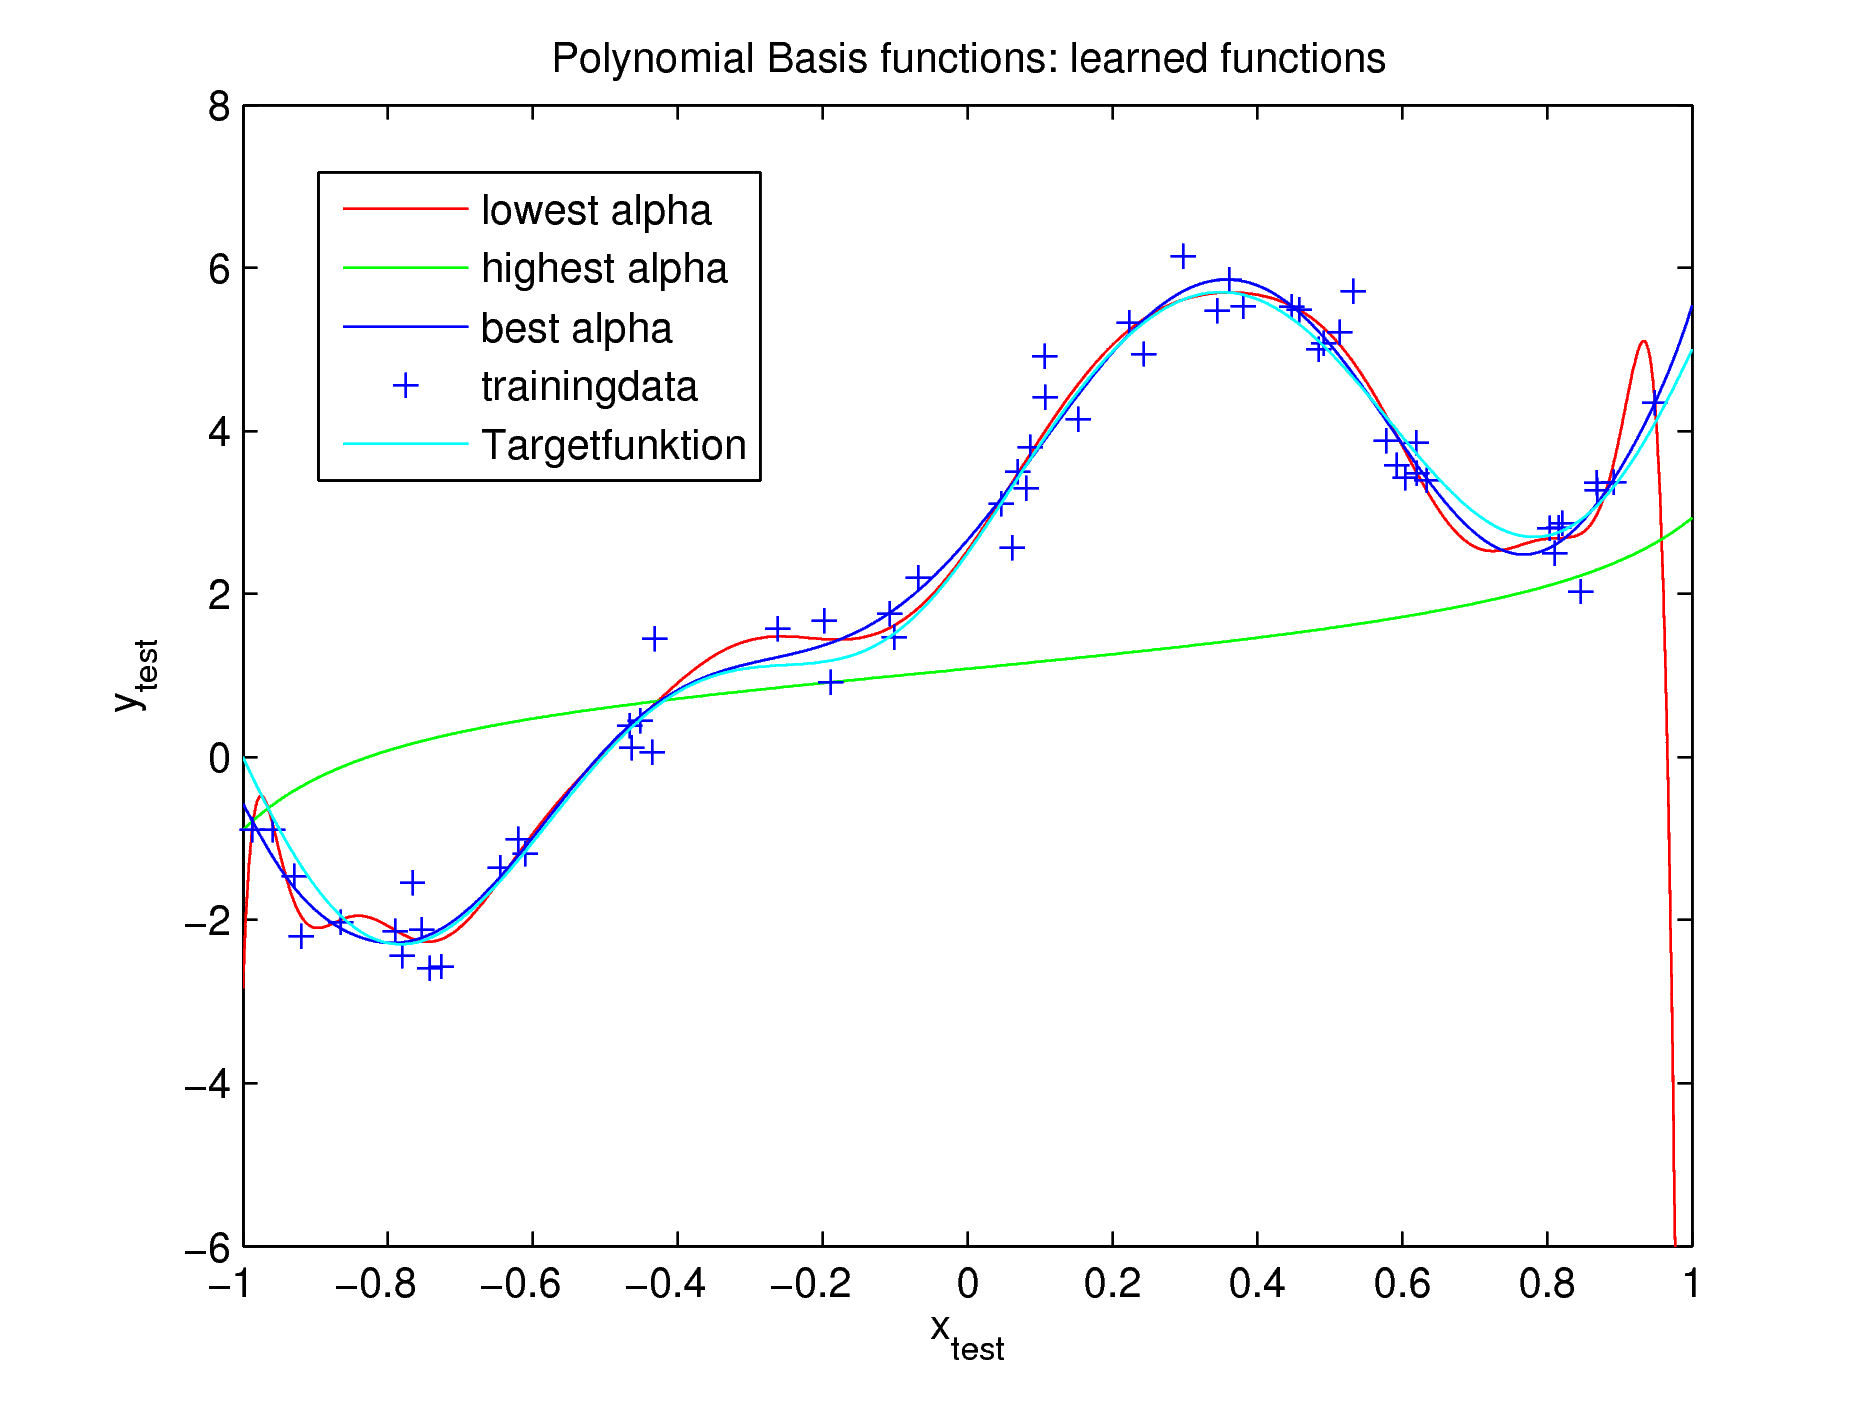
\includegraphics[width=15cm]{figures/114/poly_learned.png}
	\captionof{figure}{Polynomial Basis Functions: learned output function}
	\label{fig:poly_learned}
  \end{center}

  \begin{center}
	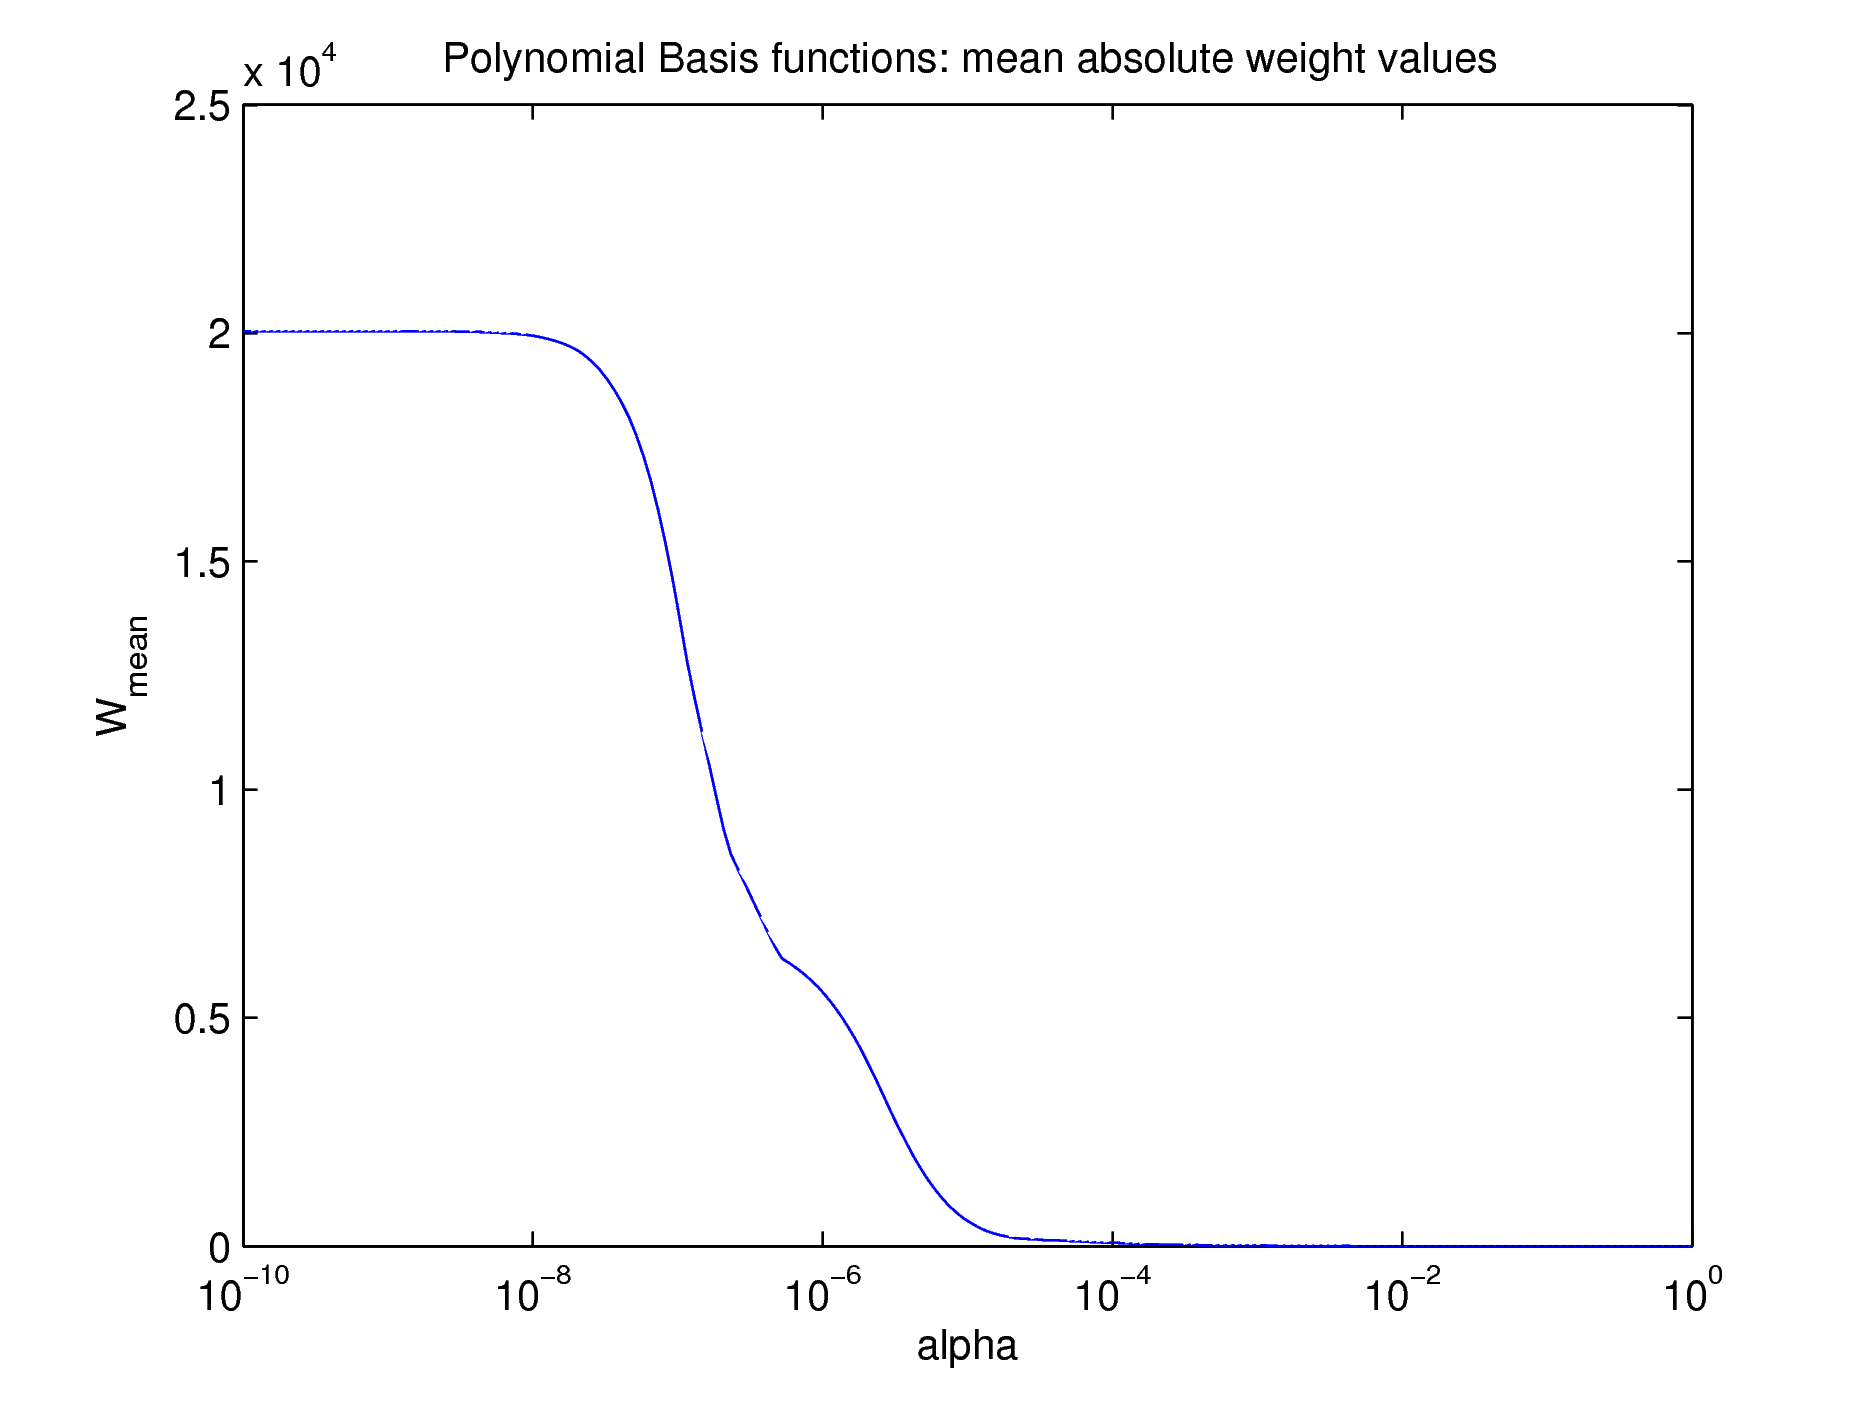
\includegraphics[width=15cm]{figures/114/poly_meanweight.png}
	\captionof{figure}{Polynomial Basis Functions: mean absolute weight over $\alpha$}
	\label{fig:poly_meanweight}
  \end{center}


\paragraph{Radial Basis Functions}

Wie in der Abbildung \ref{fig:radial_mse} zu sehen ist, ergibt sich ein minima des MSE der Testdaten
bei $\alpha = 0.021964$. Wie in der Abbildug \ref{fig:radial_learned} zu sehen ist, bewirkt ein höherer Wert von
$\alpha$ keine wesentliche Verbesserung, so wie Beispielsweise bei den polynomialen Basisfunktionen.

Der mean squared error korrelliert bei den Radialen Basisfunktionen gar nicht mit dem MSE der Testdaten, was
auch nocheinmal zum Ausdruck bringt, dass der Trick mit dem $\alpha$ fast zu keiner Verbesserung führt.
Eine mögliche Begründung dafür wäre, dass bei den Radialen Basisfunktionen auch ohne $\alpha$ die Lernkurve
an den Rändern der Testdaten nur wenig wegknickt.


  \begin{center}
	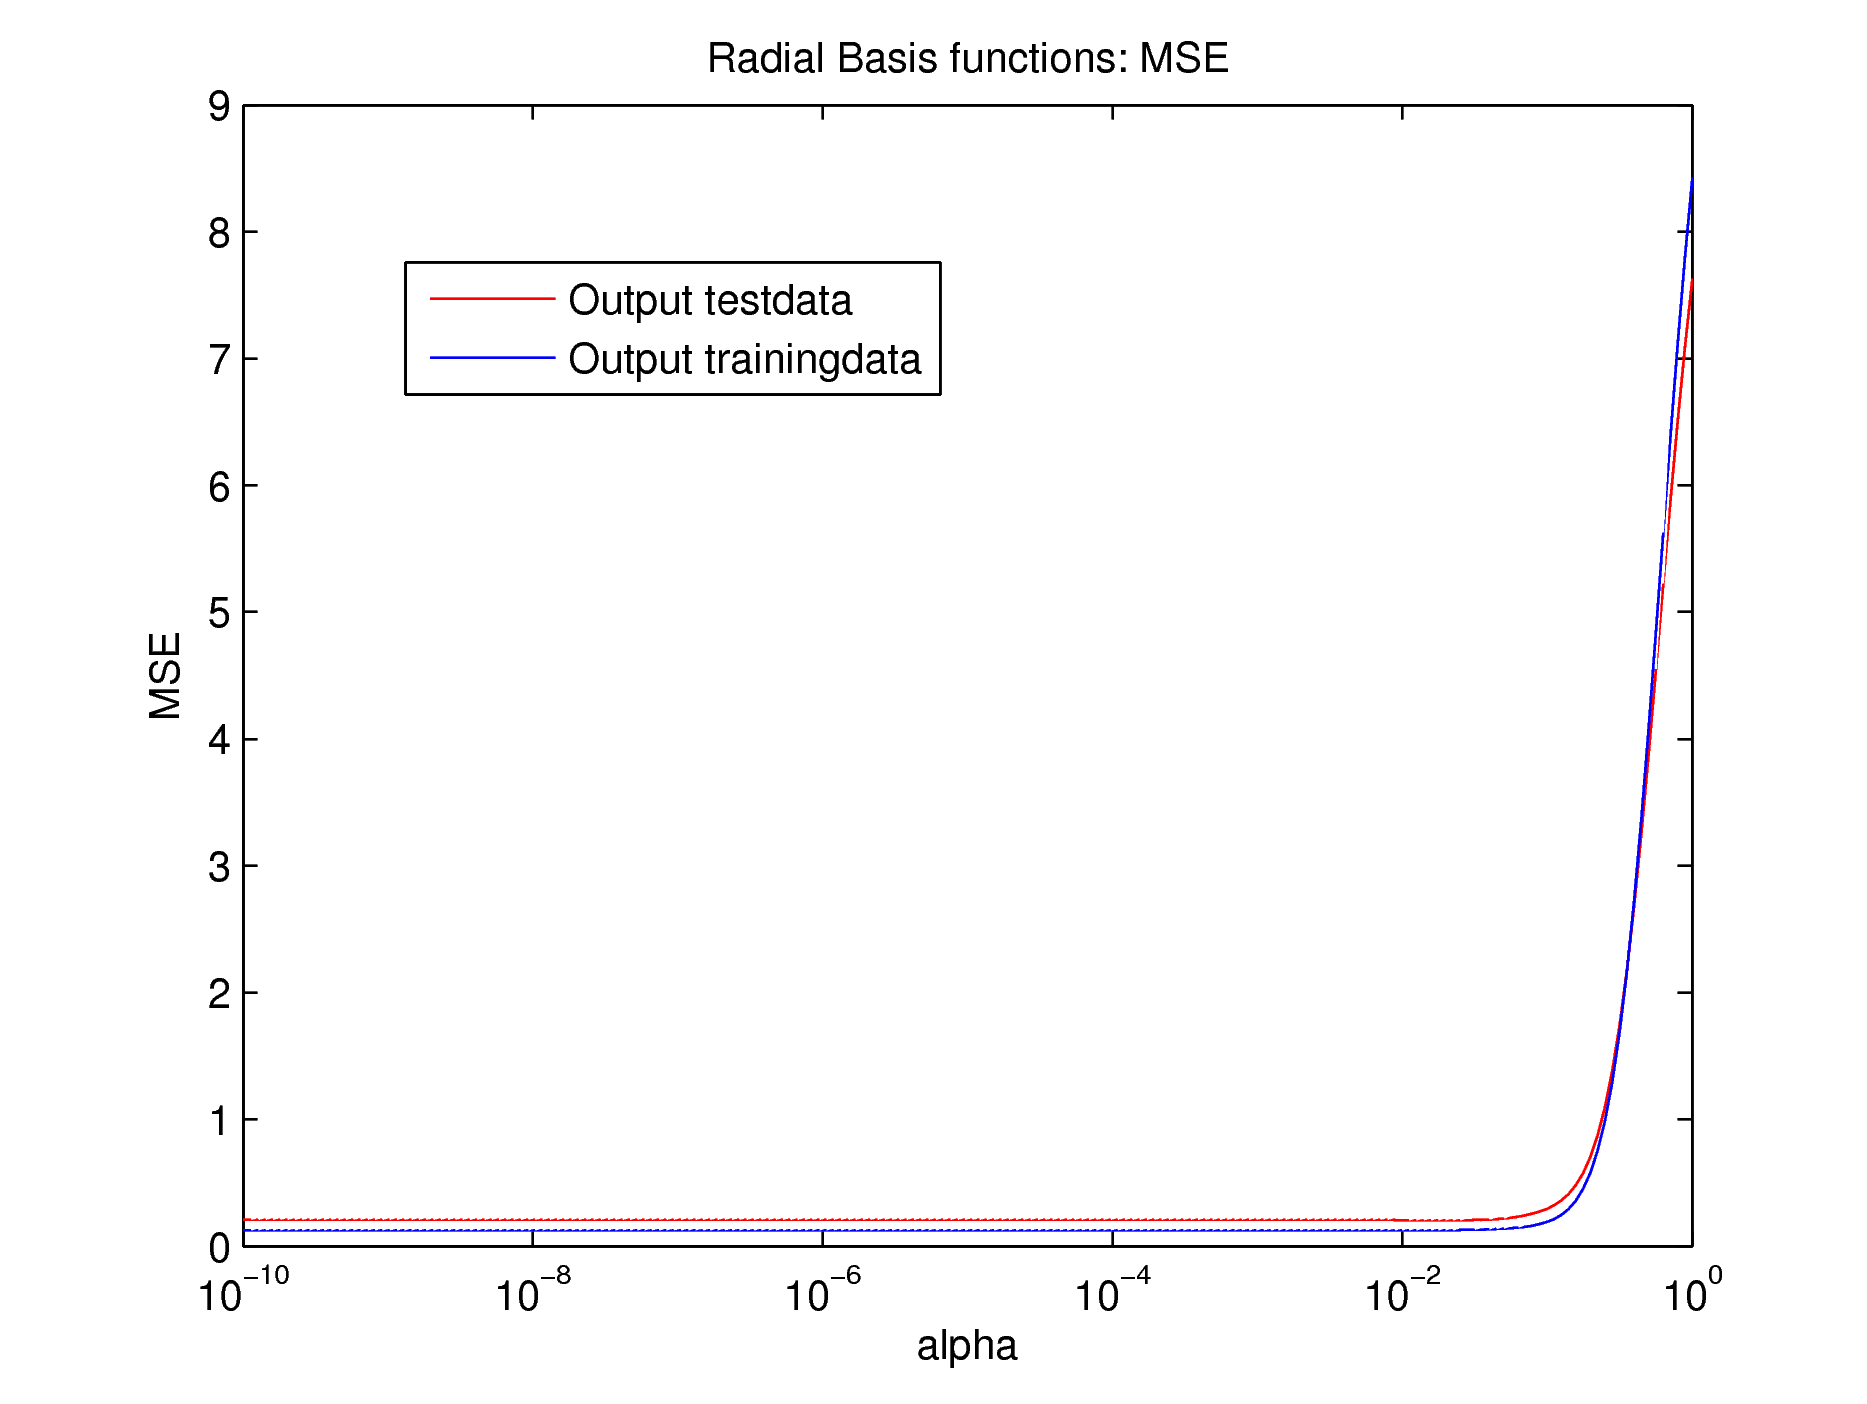
\includegraphics[width=15cm]{figures/114/radial_mse.png}
	\captionof{figure}{Radial Basis Functions: Mean squared error, Minimum bei $\alpha = 0.021964$}
	\label{fig:radial_mse}
  \end{center}

  \begin{center}
	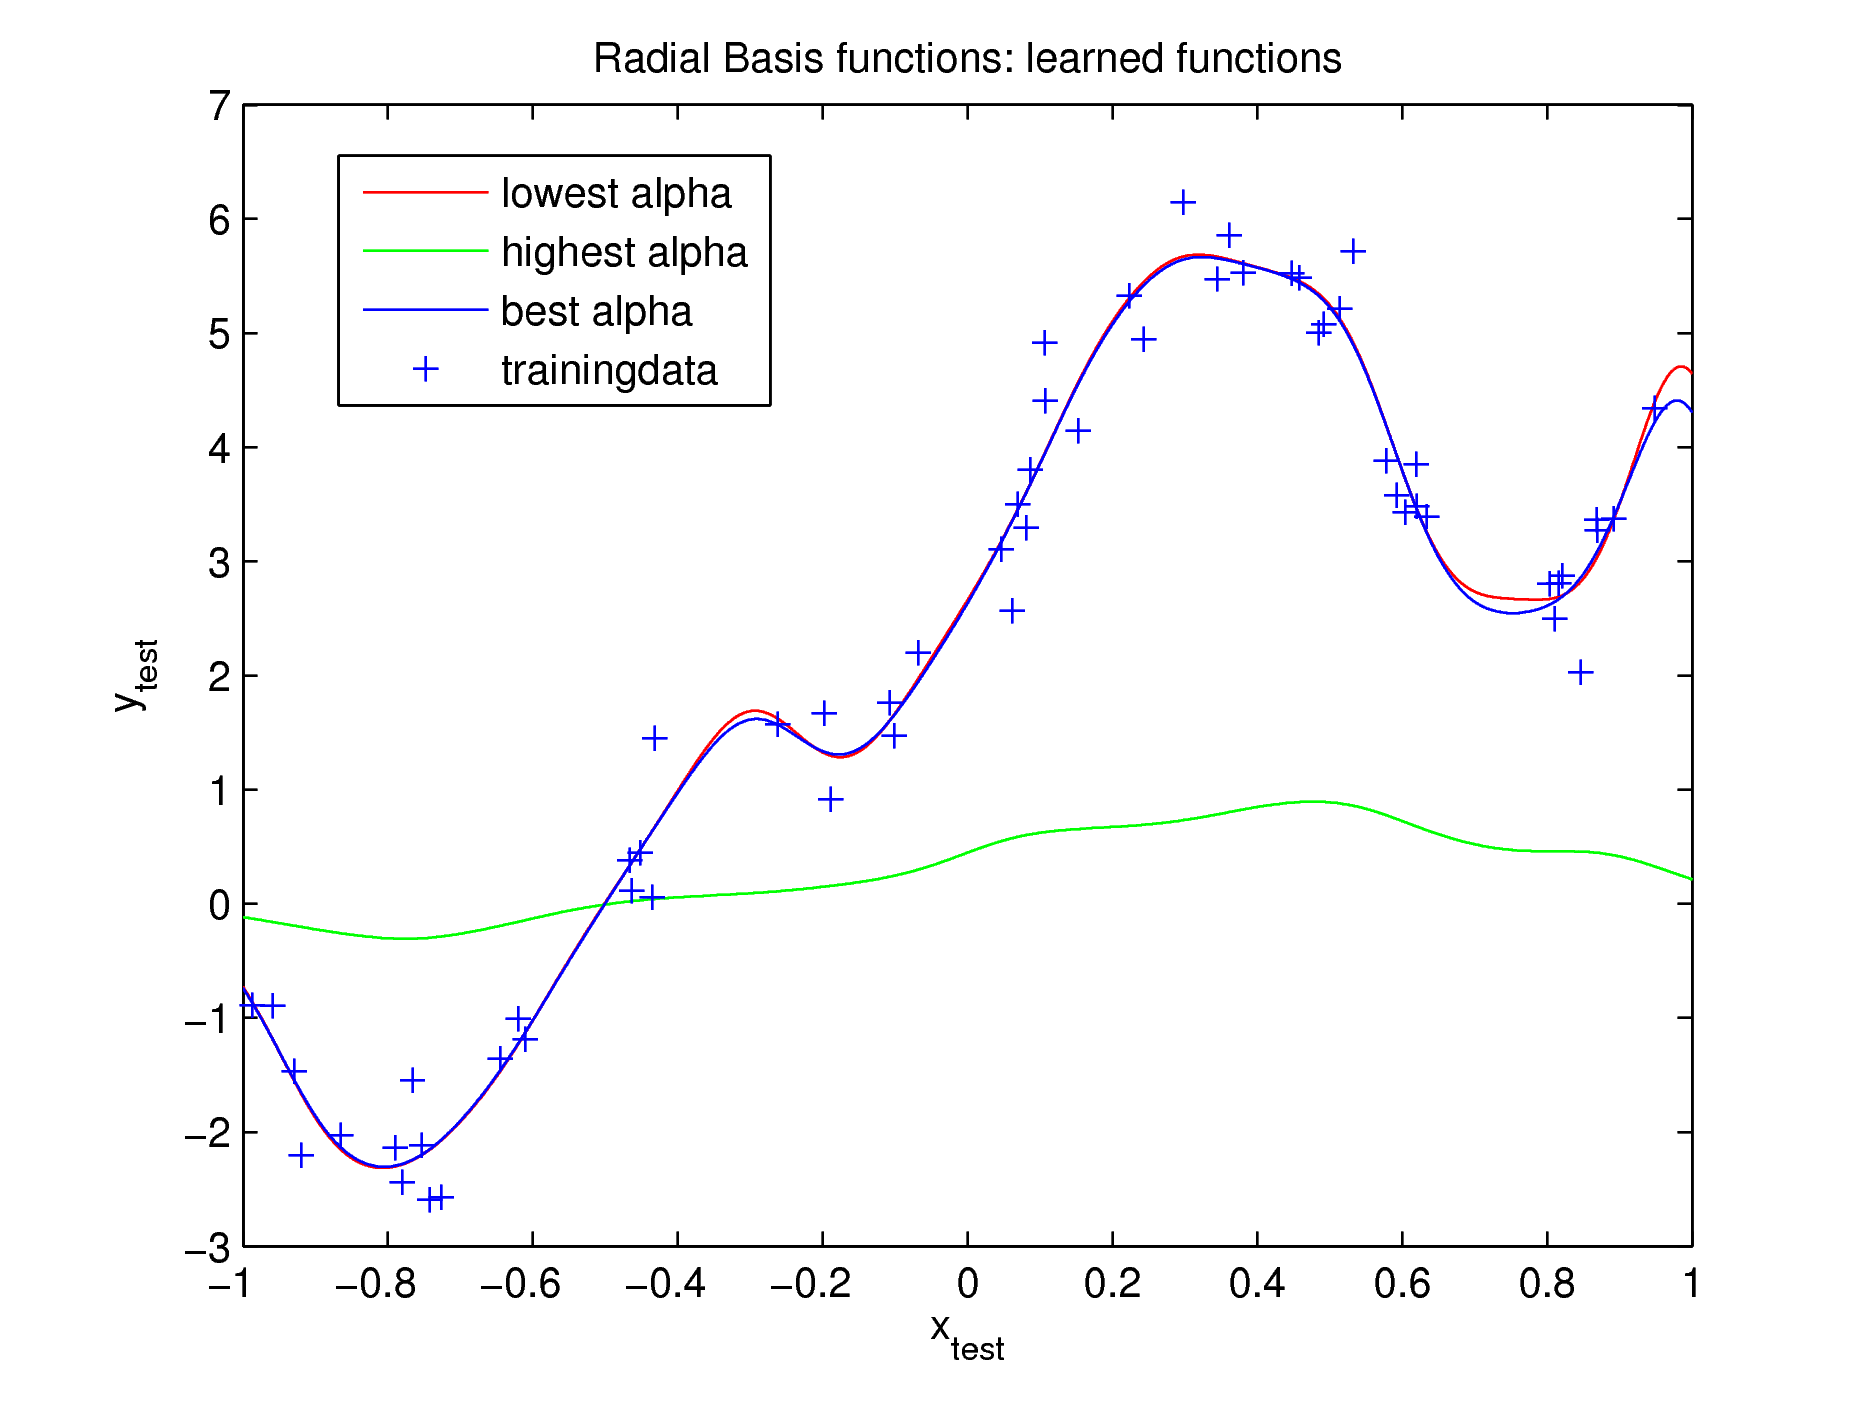
\includegraphics[width=15cm]{figures/114/radial_learned.png}
	\captionof{figure}{Radial Basis Functions: learned output function}
	\label{fig:radial_learned}
  \end{center}

  \begin{center}
	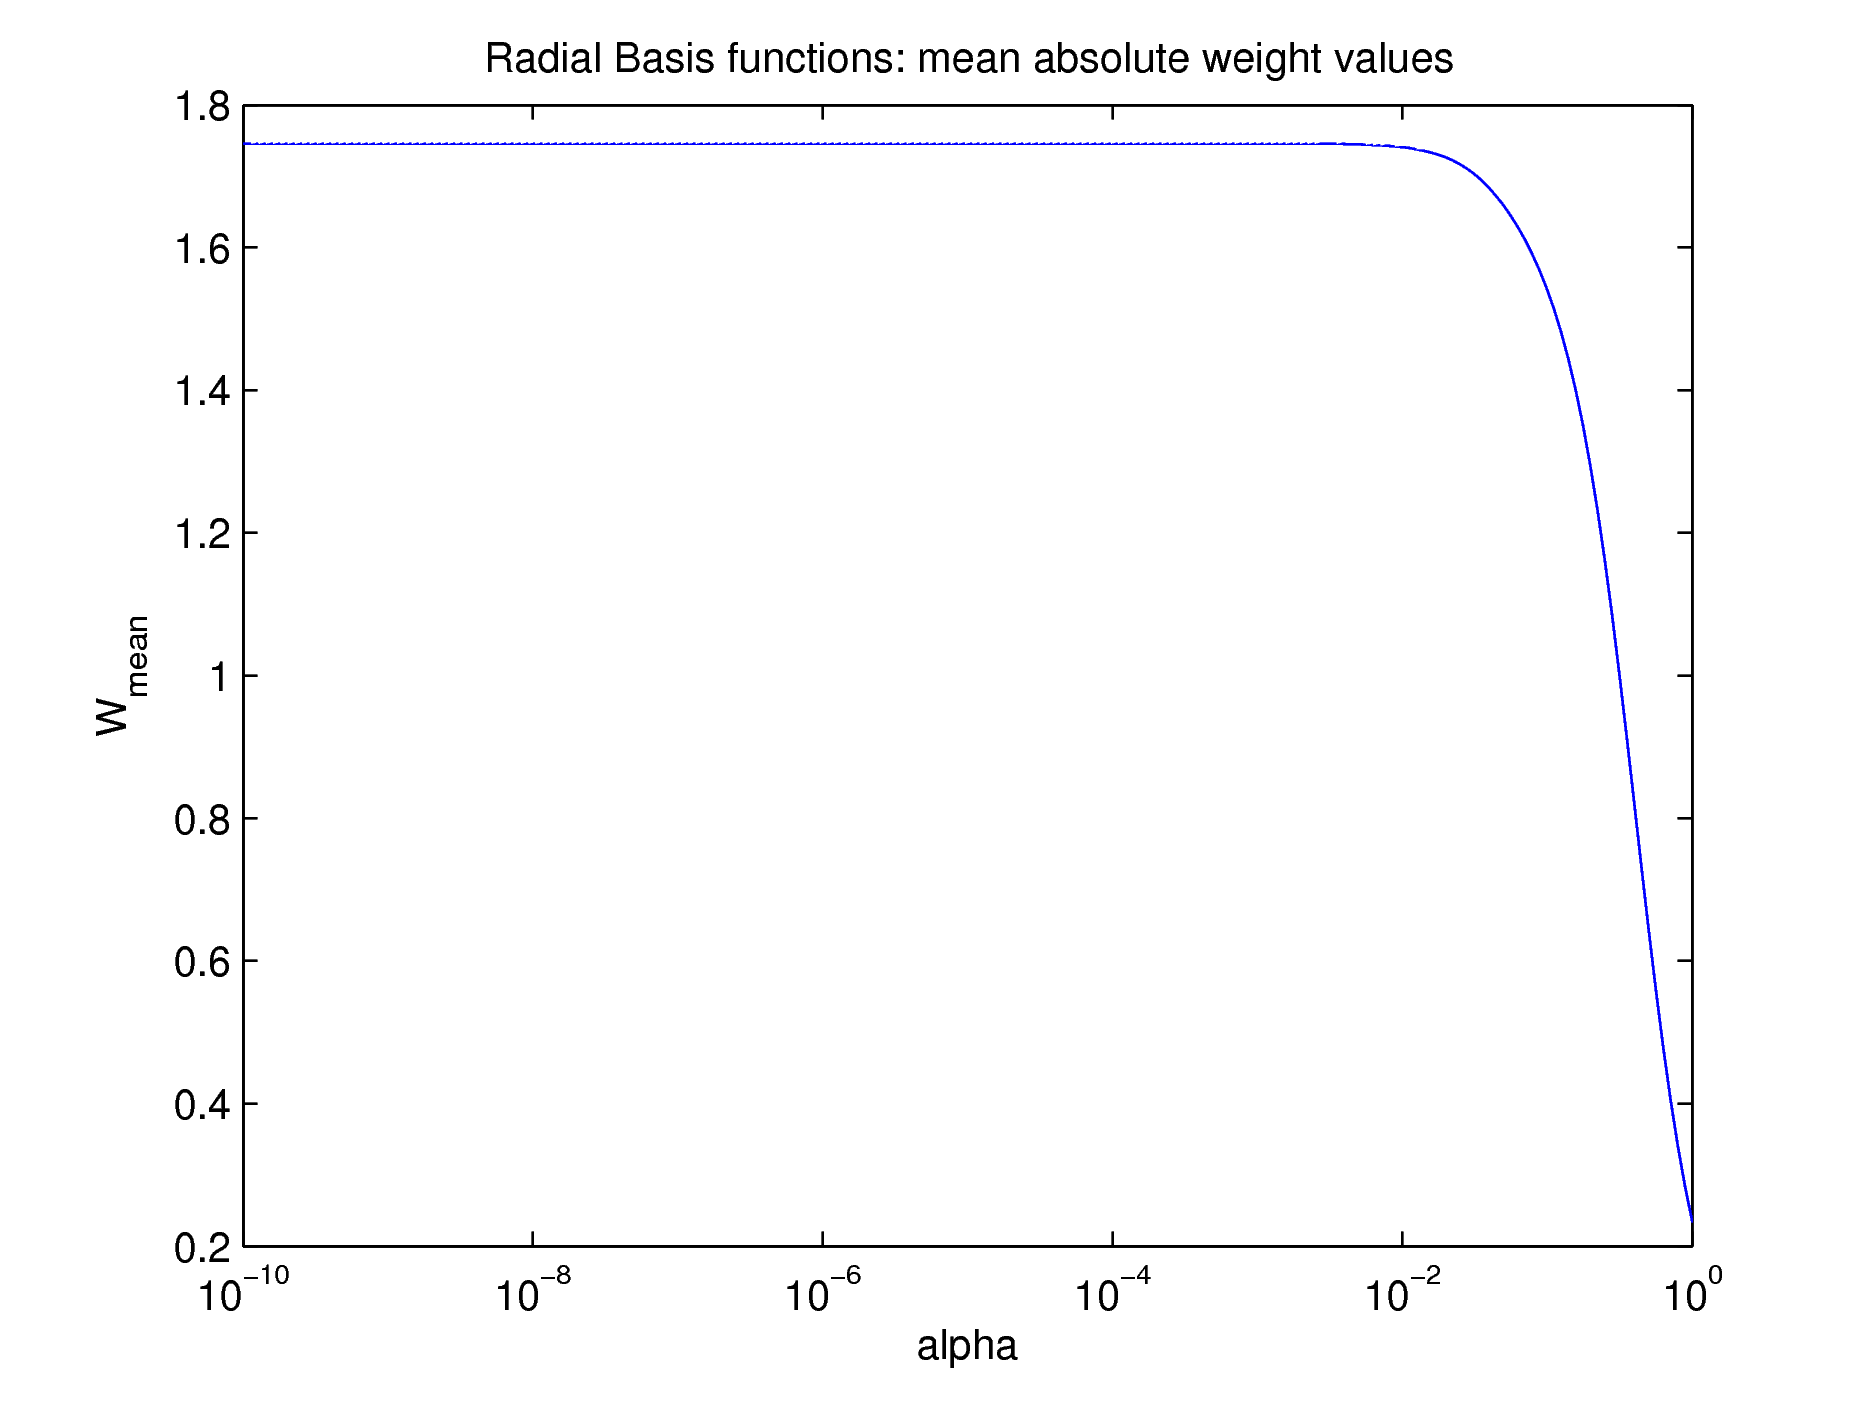
\includegraphics[width=15cm]{figures/114/radial_meanweight.png}
	\captionof{figure}{Radial Basis Functions: mean absolute weight over $\alpha$}
	\label{fig:radial_meanweight}
  \end{center}



\paragraph{Local linear models}


Wie in der Abbildung \ref{fig:local_mse} zu sehen ist, ergibt sich ein minima des MSE der Testdaten
bei $\alpha = 0.034891$. Wie in der Abbildug \ref{fig:local_learned} zu sehen ist, bewirkt ein höherer Wert von
$\alpha$ ein Abflachen der Lernkurve. Bei kleineren Werten von $\alpha$ ist die Kurve deutlich weniger abgeflacht und
folgt mehr den Trainigsdaten. Ein kleinerer Wert von $\alpha$ hat jedoch den entscheidenden Nachteil, dass ausserhalb
des Bereichs der Trainingsdaten(auf der x-Achse) und sogar zwischen größeren Abständen
zwischen den Trainingsdaten, die Lernkurve sehr stark nach oben bzw. unten wegknickt. Die Lernkurve für kleinere $\alpha$
ist eigentlich fast unbrauchbar.
$\alpha$ vergrößert bei größeren Gewichten die Fehlerfunktion $E(x)$ und wirkt somit dem entgegen.

Der mean squared error korrelliert sehr gut dem Mittelwert der absoluten Gewichte. Für Größere Werte von $\alpha$
ergibt sich verbessert sich der MSE bei den Trainings- und Testdaten. Wird jedoch $\alpha$ zu groß gewählt, so steigt
der MSE wieder.


  \begin{center}
	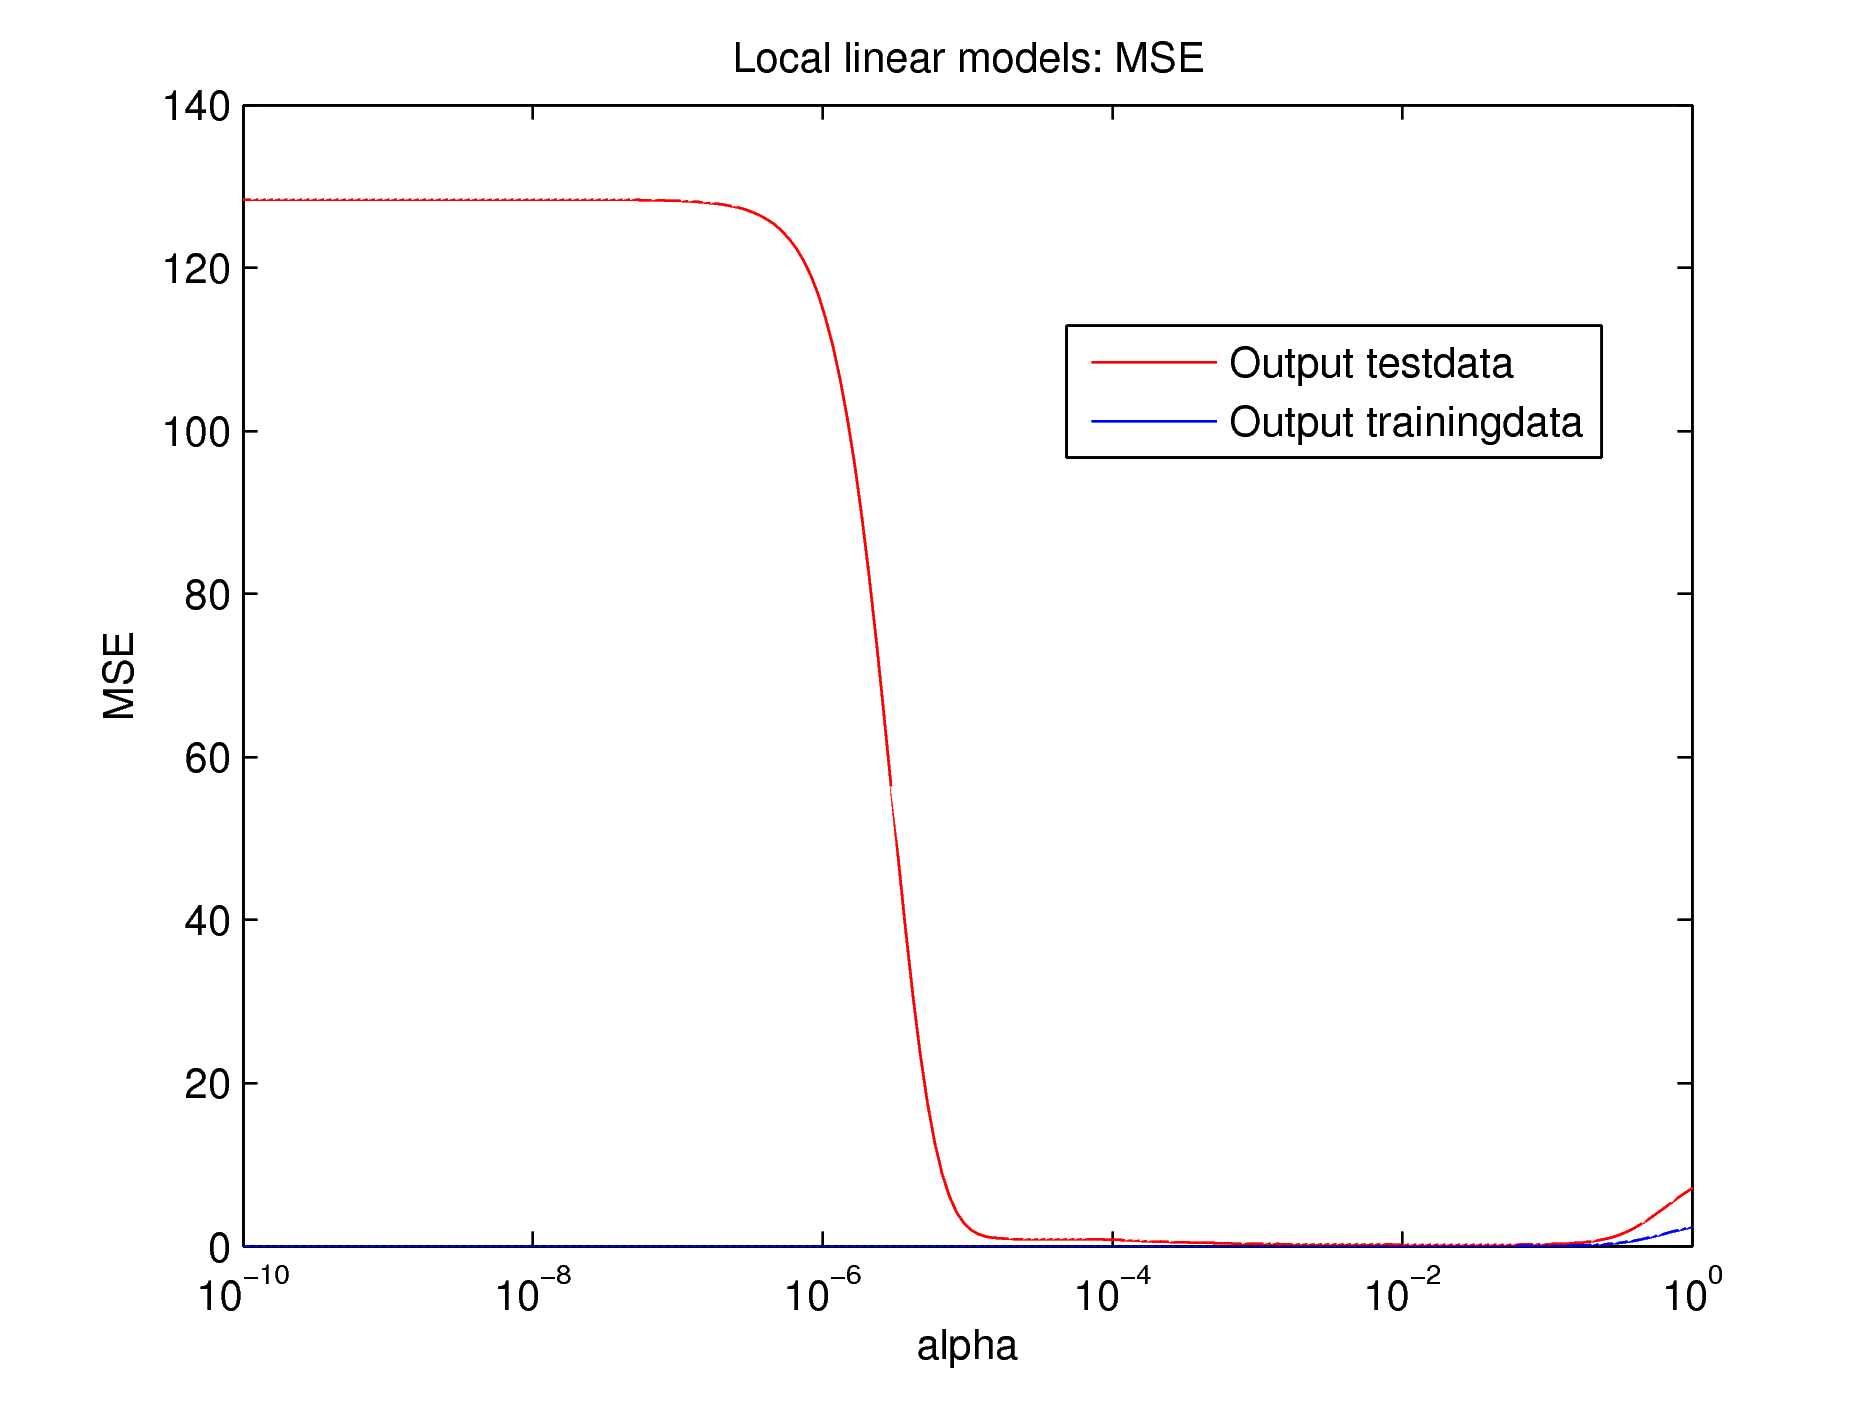
\includegraphics[width=15cm]{figures/114/local_mse.png}
	\captionof{figure}{Local linear models: Mean squared error, Minimum bei $\alpha = 0.034891$}
	\label{fig:local_mse}
  \end{center}

  \begin{center}
	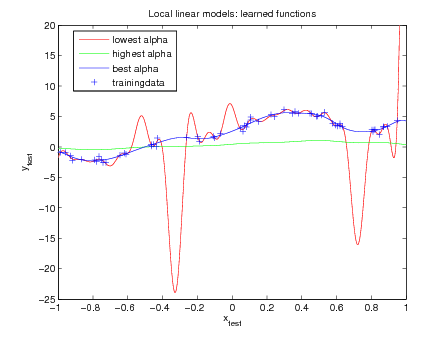
\includegraphics[width=15cm]{figures/114/local_learned.png}
	\captionof{figure}{Local linear models: learned output function}
	\label{fig:local_learned}
  \end{center}

  \begin{center}
	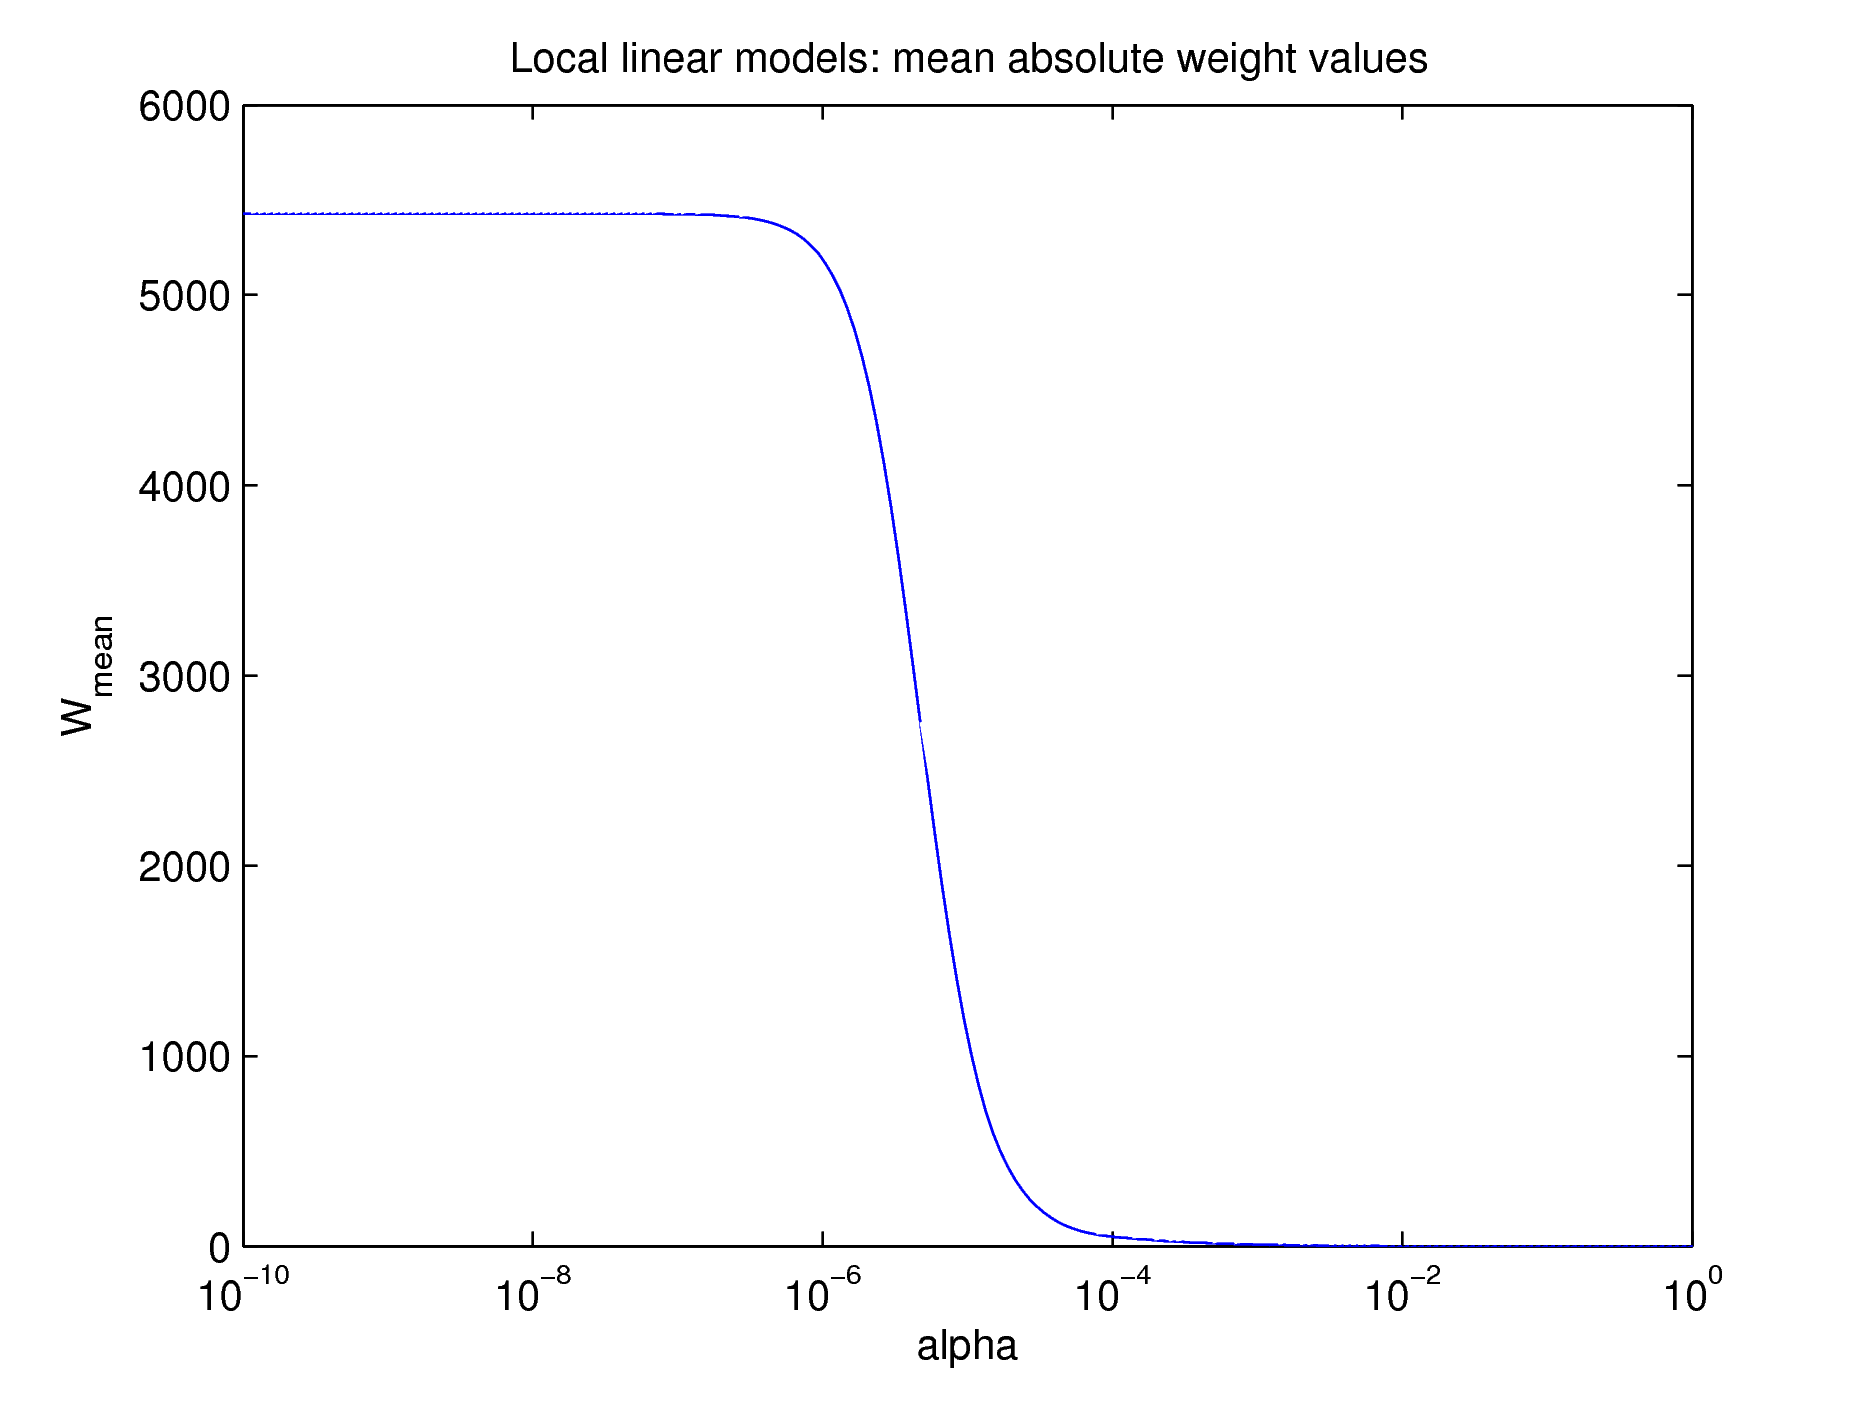
\includegraphics[width=15cm]{figures/114/local_meanweight.png}
	\captionof{figure}{Local linear models: mean absolute weight over $\alpha$}
	\label{fig:local_meanweight}
  \end{center}


\paragraph{Vergleich}

Bei den angegebenen Trainings- und Testdaten konnte mithilfe der Polynimialen Basisfunktionen das Beste
Ergebnis erzielt werden. Dabei Betrug der MSE ca. 0.189, hingegen bei den beiden anderen Verfahren ca. 0.2.
Bei Local linear Model führte der Term mit $\alpha$ zu einer deutlichen Verbesserung der Ergebnise, wobei
man bei den Radialen Basisfunktionen, den $\alpha$ - Term auch weglassen könnte ohne deutliche schlechtere
Ergebnise zu erzielen.
